\documentclass[a4paper]{oblivoir}
\usepackage{amsmath,amssymb,kotex,kswrapfig,mdframed,paralist}
\usepackage{fapapersize}
\usefapapersize{210mm,297mm,20mm,*,20mm,*}

\usepackage{tabto,pifont}
\TabPositions{0.2\textwidth,0.4\textwidth,0.6\textwidth,0.8\textwidth}
\newcommand\tabb[5]{\par\noindent
\ding{172}\:{\ensuremath{#1}}
\tab\ding{173}\:\:{\ensuremath{#2}}
\tab\ding{174}\:\:{\ensuremath{#3}}
\tab\ding{175}\:\:{\ensuremath{#4}}
\tab\ding{176}\:\:{\ensuremath{#5}}}

\usepackage{graphicx}

\pagestyle{empty}

%%% Counters
\newcounter{num}

%%% Commands
\newcommand\prob[1]
{\bigskip\par\noindent\stepcounter{num} \textbf{문제 \thenum) #1}\par\noindent}

\newcommand\pb[1]{\ensuremath{\fbox{\phantom{#1}}}}

\newcommand\ba{\ensuremath{\:|\:}}

\newcommand\vs[1]{\vspace{25pt}}

\newcommand\an[1]{\bigskip\par\noindent\textbf{문제 #1)}\par\noindent}

%%% Meta Commands
\let\oldsection\section
\renewcommand\section{\clearpage\oldsection}

\let\emph\textsf

\begin{document}
\begin{center}
\LARGE준영, 미니테스트 13
\end{center}
\begin{flushright}
날짜 : 2017년 \(\pb3\)월 \(\pb{10}\)일 \(\pb{월}\)요일
,\qquad
제한시간 : \pb{17년}분
,\qquad
점수 : \pb{20} / \pb{20}
\end{flushright}

%
\prob{}
다음 빈칸에 알맞은 것을 넣어라.
\begin{enumerate}[(1)]
\item
\(\displaystyle\lim_{x\to1}f(x)\text{가 존재한다.}\iff
\fbox{\phantom{\(\displaystyle\lim_{x\to1+}f(x)\)}}
=
\fbox{\phantom{\(\displaystyle\lim_{x\to1-}f(x)\)}}
\)
\item
\(f(x)\text{가 }x=1\text{에서 연속이다.}\iff
\fbox{\phantom{\(\displaystyle\lim_{x\to1}f(x)\)}}
=
\fbox{\phantom{\(f(1)\)}}
\)
\item
\(f(x)\text{가 }x=1\text{에서 미분가능하다.}\iff
\fbox{\phantom{f'(1)}}\text{이 존재한다.}\)
\end{enumerate}

%
\prob{}
함수 \(f(x)=\frac{x^2(x-2)}{x-2}\)에 대해 다음 물음에 답하여라.
\begin{enumerate}[(1)]
\item
이 함수의 정의역은 \(\{x\,|\,x\text{는  }\fbox{\phantom{\(x\neq0\)}}\text{인 실수}\}\) 이다.
\item
이 함수의 그래프를 그려라.\\
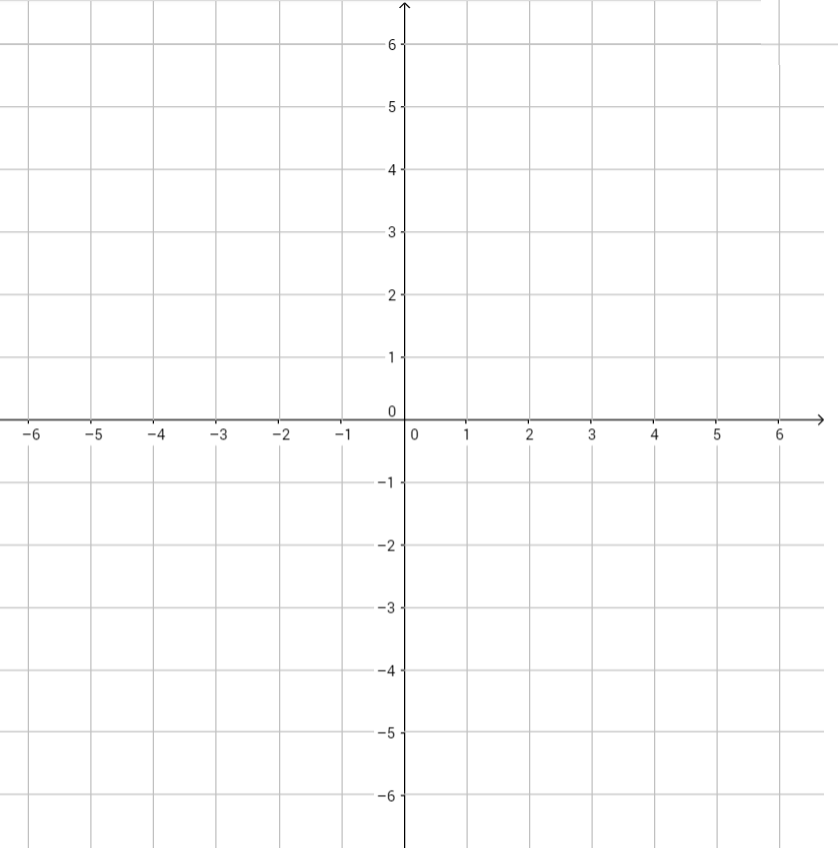
\includegraphics[width=0.6\textwidth]{graph_paper}
\item
\(\displaystyle\lim_{x\to2}f(x)\)가 존재한다 / 존재하지 않는다. (존재하면 극한값도 구하여라.)
\item
\(f(x)\)가 \(x=2\)에서 연속이다 / 불연속이다.
\item
\(f(x)\)가 \(x=2\)에서 미분가능하다 / 미분불가능하다. (미분가능하면 미분계수도 구하여라.)
\item
\(\displaystyle\lim_{x\to-1}f(x)\)가 존재한다 / 존재하지 않는다. (존재하면 극한값도 구하여라.)
\item
\(f(x)\)가 \(x=-1\)에서 연속이다 / 불연속이다.
\item
\(f(x)\)가 \(x=-1\)에서 미분가능하다 / 미분불가능하다. (미분가능하면 미분계수도 구하여라.)
\end{enumerate}
\end{document}